\chapter{Pre and post processing work preparation}
\label{Chapter2}

\section{Introduction}

To complete

\section{Tools used during the test}

\subsection{MMCG test piece}

The MMCG test piece was developed by Moutou Piti [MOU 2008]. However, the specimens tested at the University of Lisbon are not of the same dimensions. After carefully measuring the specimens, it turns out that they have the same dimensions as the specimens studied by Odounga. Below are the dimensions of the specimens that will be tested figure \ref{fig:fig23}:

\graphicspath{{Images/}}
\begin{figure}[htp]
	\centering
	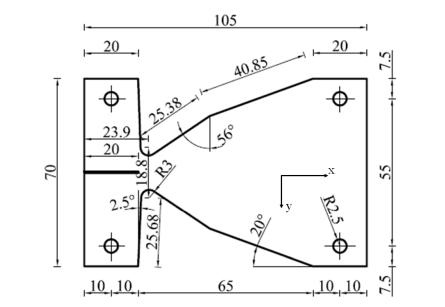
\includegraphics[width=8cm]{fig23}
	\caption{Dimensions of the tested MMCG specimen}
	\label{fig:fig23}
\end{figure}

\subsection{Arcan model and final grips}

To perform the tests, a steel Arcan system must be designed. It is made of high tensile steel (HLE). Indeed, this part allows to connect the 2MCG wood specimen to the press. In order to create this grip we must first take into account the dimensions of the 2MCG specimen available in Nova school described in figure \ref{fig:fig24}. The shape of the Arcan system must also allow a good visibility on the propagation of the crack. Figure 21 shows the Arcan device that we will use, which was inspired from the thesis of [ODO 2018].

\graphicspath{{Images/}}
\begin{figure}[htp]
	\centering
	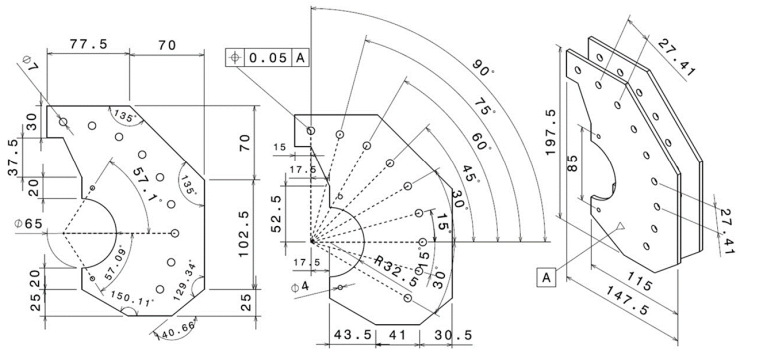
\includegraphics[width=10cm]{fig24}
	\caption{Size of the Arcan fastening system[ODO 2018]}
	\label{fig:fig24}
\end{figure}

The fixing holes for the wooden specimens have a diameter $\Phi= 5 mm$, and the loading holes have a diameter $\Phi = 7 mm$. These fixing holes were drilled in order to be able to load the specimen with different angular values of the angle in relation to the vertical direction in order to activate different failure modes depending on the load angle. To connect the Arcan system to the press, a piece had to be created, as shown in figure \ref{fig:fig25}.

\graphicspath{{Images/}}
\begin{figure}[htp]
	\centering
	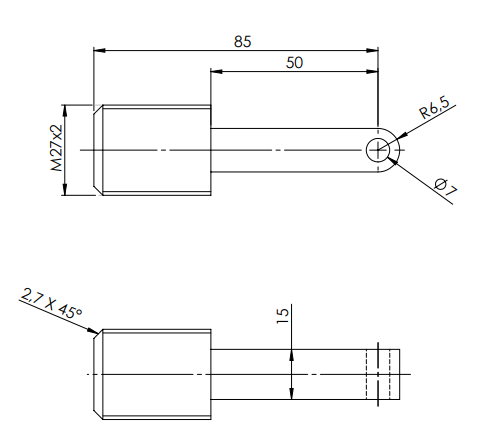
\includegraphics[width=6cm]{fig25}
	\caption{Bolt for connecting the press and the Arcan System}
	\label{fig:fig25}
\end{figure}

This part has a hole of the same size as the holes of the Arcan system in order to connect them. Moreover the head of the connector is 27mm in diameter and the thread has a 2mm pitch to connect to the press. Before sending the technical drawings to a company, a 3D printer was used to verify that the system worked properly. It was then necessary to draw the assembly on solidworks in order to print the assembly and send the technical drawings. Figure \ref{fig:fig26} shows the assembled device in Solidworks.

\graphicspath{{Images/}}
\begin{figure}[htp]
	\centering
	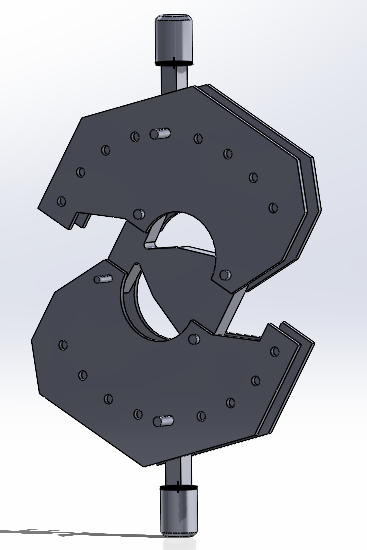
\includegraphics[width=5cm]{fig26}
	\caption{Assembled device in Solidworks}
	\label{fig:fig26}
\end{figure}

It has been shown in previous work such as [ODO 2018] that one of the main problems with the MMCG specimen is the small distance between the holes and specimen extremities. This implies several cracks in the heel between the hole and the extremity of the sample which prevents observation and analysis of the fracture. One solution proposed by Odounga is the use of washers which could be glued or to strength screw the nut. Indeed, by applying compressive stress on each side of the sample, it reduces the stress applied on the holes and distributes the load in a wider area.

\subsection{Hydraulic press used}

To determine experimental parameters like the load speed or the frequency of the camera recording, it was important to read previous works on the subject and determine which engines will be used to proceed the experiments. The press used for the tests is a Landmark Servohydraulic Test Systems model 661.21B-03  from MTS. It is capable of exerting a maximal applied load of 10 metric to N (figure \ref{fig:fig27}).
In the work of Ostapska and Malo [KAT 2021] the load speed recommended was about $0.1\ mm\ {min}^{-1}$ and the record was made at a frequency of 5 Hz, so 5 images per seconds. In the work of Mambili the record was made at a frequency of 10 Hz and the load speed was about 0.3 mm/s with a pre-load of 100N. It should be remembered that this press is also chosen because of its ability to load the specimens with a constant time displacement. Indeed, it was explained that this work will use the complacency method to compare the results.

As explained Stanislas Malfait [MAL 2021]  this MTS Hydraulic Press works with a cooler fluid. Indeed, a tank full of fluid mixed to water and a cooler system send this fluid mix to the press as visible on 23. Then, a hydraulic supply from MTS sends this liquid to the press itself. It is the model 506.02 serie 22 coupled with the Vickers DG4V-3-2A. Then the pressure is created thanks to the Hydraulic Service Manifold part from MTS company, model 234.11. Finally, a servo valve MOOG A076-263c increase the pressure to allow the hydraulic press operation. It is a high performance valve which drives a dry torque motor. Then a MTS load cell (661-21B-03) allows to follow the displacement of the hydraulic press.

\graphicspath{{Images/}}
\begin{figure}[htp]
	\centering
	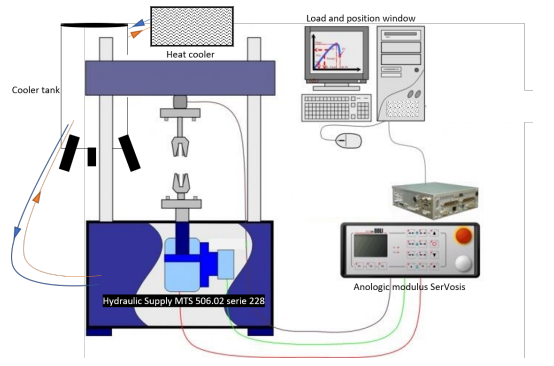
\includegraphics[width=10cm]{fig27}
	\caption{Hydraulic Press components allowing it use[MAL 2021]}
	\label{fig:fig27}
\end{figure}

\section{Research and understanding of the parameters of the DIC method}

\subsection{Characteristic of the Wood used}

In this section, the values of the mechanical characteristics (moduli of elasticity, compliances and shear coefficients) are given. As no characterization tests were carried out in this study, the data from the literature are used here, following the document created by Guitard\cite{Reference20}. These values which are the shearing $G_{ij}$ and longitudinal modulus $E_i$ , the Poisson’s coefficient $\nu_{ij}$ and $\rho$ change for each species. Moreover, these values can evolve due to temperature and relative humidity. By knowing the temperature, the relative humidity and the volume weight of a specimen, it is possible to obtain the characteristics wanted. Table \ref{fig:fig28} and \ref{fig:fig29} give us the characteristics for the Pinus Sp Pine at 9.7$\%$ humidity:

\graphicspath{{Images/}}
\begin{table}[htp]
	\centering
	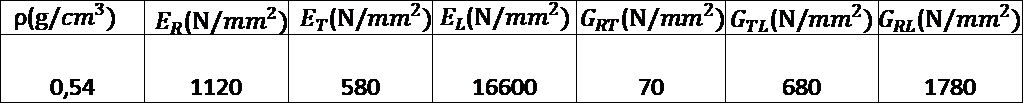
\includegraphics[width=10cm]{fig28}
	\caption{Characteristic of the Pinus Sp Pine}
	\label{fig:fig28}
\end{table}

\graphicspath{{Images/}}
\begin{table}[htp]
	\centering
	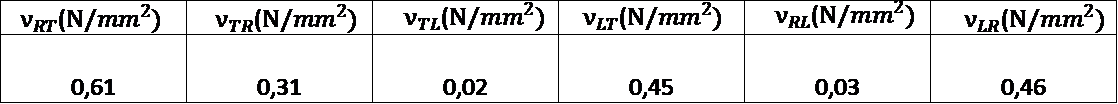
\includegraphics[width=10cm]{fig29}
	\caption{Characteristic of the Pinus Sp Pine}
	\label{fig:fig29}
\end{table}

\subsection{Preparation of the DIC method}

Before starting the measurements with the DIC method, it is important to define some parameters. In our case, the quantity of interest is the crack length a as a function of the applied force F. It is also important to define the zone of interest (ZOI). It is the portion of the image corresponding to the zone-of-interest of the test piece.. The field of view ( FOV), the position envelope for hardware and if the test is a 2D-DIC or a stereo DIC are parameters to take into account. In our case, a 2D-DIC is suitable because the test piece is assumed to be planar and perpendicular to the camera optical axis. The camera and lens have to be well selected in order to obtain the desired FOV and spatial resolution for example. With a pre-determined aperture of the lens, it’s important to select lighting and an exposure time to have sufficient contrast between the white and black regions of the DIC pattern. The contrast should be uniform over the entire ZOI of the image and constant in time. The DIC pattern is one important parameter. All the specimens are painted to obtain a speckle pattern suitable for image correlation. A thin layer of white paint is firstly added using a mate spray, followed by a diffuse distribution of black paint to create a unique local pattern across the ZOI at the crack tip. Estimate the spatial gradients which means determine such as the subset size and the step size. This will determine the required spatial resolution of the DIC system. It’s also necessary to determine the acceptable noise floor and the frame rate. The DIC images need to be synchronized to the force applied by the press. To finish, the calibration must be done. The goal of calibration of a 2D-DIC system is to establish the image scale, i.e. the number of pixels in the image that corresponds to a certain physical distance on the test piece, and to correct for lens distortions.

\subsection{MatchID}

Once the tests are completed, the data is saved on a hard disk for processing. It is possible to process the images with different software. Mambili used Ncorr and matlab while Stanislas Malfait used MatchID and Python. This image processing will allow to obtain the maps of deformations and displacements. For this work will be used matchid and python.

With the MatchID software several steps are necessary:

\begin{itemize}
	\item Choose a reference image that corresponds to the first image of the test 
	\item Select multiple deformed images
	\item Define the zone of interest (ZOI) in which the crack propagates
	\item Define the analysis parameters of the ZOI
	\item Start the DIC analysis
	\item Exploit the results
\end{itemize}

Despite the progress and increasing use of DIC, the technique is still not standardized. It is emphasized that extrinsic and intrinsic DIC setup parameters, such as subset size, subset step, strain gauge window, shape functions, or correlation criterion, can have a considerable influence on the calculated strain fields, producing spatial resolution and resolution values that can differ by at least an order of magnitude. This paragraph will try to explain some of them. 

The correlation criterion defines the matching criterion that will be adopted in order to determine the optimum corresponding point. \cite{Reference10}  used the criterion ZNSSD. It is a least-square-based correlation criterion which is less sensitive to both image contrast reduction and light intensity shifting between images. 
There are 5 subset shape function which allow or not the subset certain constraints as the fact of translating, deforming, to shear etc.. Depending on the local deformation or strain gradients of the problem under analysis, affine, irregular and quadratic shape functions can be selected by the user in the DIC method \cite{Reference21}. The subset size is the length of the subset in the reference image and it must contain at least 3 speckles. As an indication, larger subsets improve resolution but decrease spatial resolution. This means that in a conventional mechanical tensile test with a uniform, uniaxial stress state in the central region of the specimen, large subsets can be selected to improve the accuracy of the measurements. The step size is the spacing of pixel grid points at which the subset displacements are calculated. It controls the density of points at which DIC data is computed and, to some extent, influences the spatial resolution of the measurements. Typically, a step size of one-third to one-half of the subset size is recommended, so that neighboring subsets partially overlap, though this value can vary widely depending on specific applications. Additionally, a small step size may be required to capture the peak position of a Quantity Of Interest (QOI) (without interpolation) if it varies quickly across the ZOI and if the QOI varies slowly across the ZOI, then a large step size can be used. The strain window is the local region of the ZOI of the image, containing a finite number of data points, that is used to calculate strain. Parameters such as the subset step and the strain window will define a strain spatial resolution and virtual strain gauge (VSG). VSG is the local region of the image that affects the strain value at a specific location. The three dominant variables that affect the VSG size are the subset size, step size, and strain window. If the maximum strain amplitude converges with further decreases of the VSG, then the actual maximum strain amplitude has been captured. Any VSG that is larger than the largest VSG that results in the converged actual maximum strain amplitude will underestimate the actual strain amplitude, and introduce bias into the measured strain results. If the smallest VSG allowed by the software is not sufficient, the test could be repeated with a smaller FOV. The final decision as to which size VSG to use is a matter of judgment. If capturing the highest strain gradient is essential for DIC analysis, a small VSG may be the best choice, even if noise is important. Conversely, if there are no high strain gradients it may be preferable to choose a larger VSG to reduce uncertainties. In order to determine the correct settings MatchID has a tool called Performance Analysis. With this tool, it’s possible to define a range of options to be applied in a design of experiments study. It is thus possible to vary parameters such as subset size, step size, strain window and so on. After running the performance analysis, select the parameters which work best(video 20). For the case of a uniaxial tensile test on a pre-cracked specimen by default the indicated zone of interest contains one initial subset but the ZOI is not well defined. In order to define well the ZOI it must be added an extra seed point in the ZOI but above the initial crack. After this, start the DIC analysis and exploit the results. To exploit the results in MatchID, it is possible to import data. In this case, import the data on the force applied throughout the test in order to plot the force as a function of the displacements for example (video 11).

\subsection{Uncertainty Quantification}

There are two types of errors in DIC measurements, namely variance errors and bias errors. The main sources of noise in DIC measurements are camera noise and matching errors during the correlation process. Bias can be introduced by smoothing of spatial gradients in a QOI, uncorrected lens distortions, poor camera calibration, and out-of-plane motion in 2D-DIC measurements, to name a few sources. Establishing the uncertainty of the QOIs accounting for bias and noise errors is essential for intelligent evaluation and use of DIC results. Without quantifying the uncertainty, it is impossible to know whether a reported QOI value is meaningful and relevant, or whether it is the result of random noise and bias.

Bias errors are often difficult to quantify, as the true value of a QOI is usually not known. However, some sources of bias can be assessed. Even if no bias errors are detected, unknown bias errors may still exist!

The process of quantifying variance errors is often called noise floor analysis. The basic idea of a noise floor analysis is to correlate static images of a DIC pattern that were acquired under the same conditions as the test images. With no force applied or displacement on the test piece, all measured QOIs requiring deformation are errors. The evaluation of the noise floor must be performed under the same conditions as the mechanical test, both in terms of physical conditions (camera and lens selection, illumination, camera temperature, cooling or mixing fans, powered test machine) and data processing procedures (image pre-filtering, subset size, step size, VSG size, temporal or spatial filtering of the data, etc.). This means that the same user-selected DIC parameters that are used for the analysis of the test piece images during deformation should also be used for the analysis of the noise floor images. Therefore, the final noise floor analysis is typically performed after the mechanical test image analysis, but using the images acquired immediately before the mechanical test.
Two different metrics can be used to quantify the variance error of the QOIs: a spatial standard deviation and a temporal standard deviation. To quantify the spatial variation of the QOI, compute the standard deviation of the QOI for each image and average this spatial standard deviation over time for all static images. To quantify temporal variation, calculate the standard deviation of the QOI for each subset over time and average this temporal standard deviation for each subset over all subsets in the image ZOI. It is recommended that both spatial and temporal standard deviations be calculated and evaluated to see if one is significantly larger than the other. However, the spatial and temporal standard deviations are generally similar, and a single metric or the average of the two metrics can be selected to quantify the noise floor. 

\section{Python}

Python is a computer programming language often used to create websites and software, automate tasks and perform data analysis. It is a versatile language, which means that it can be used to create a variety of different programs and is not specialized for specific problems. This versatility, along with its beginner-friendliness, has made it one of the most widely used programming languages today.

A second data processing is necessary to obtain the position of the crack front and the displacements. Below are the processing steps:

\textbf{Crack opening displacement (COD) or Virtual displacement}

From the reference and current positions of the DIC calculation points, the Euclidean distance between each pair of points can be measured and the COD can be determined as follow:

\begin{equation}
	VD(k,i_n)=\sqrt{(x_{11bk}-x_{11tk})^2 + (x_{22bk}-x_{22tk})^2}_{i_n} - VD(k,i_0)
\end{equation}

where the indices t and b refer to the DIC data points located at the top and bottom of the crack path, k is the index of the DIC point, in is the image captured at time n, VD(k, i0) is the initial Euclidean distance between the computational points of the top and bottom reference DIC subset obtained from image i0, and $x_{11}$ and $x_{22}$ are their coordinates in the image plane.

\textbf{$\alpha$ and $\beta$ parameters}

Two kinds of techniques as an integer value representing the threshold can be used:

The first one uses just the parameter $\alpha$ which is selected as the lowest integer satisfying the inequality:

\begin{equation}
	a(\alpha)-a_0 < f_s, \alpha \in \mathbb{N}
\end{equation}

where fs is the spatial resolution associated to DIC measurements.

The second uses 2 parameters $\alpha$ and $\beta$ which are defined below:

\begin{equation}
	\alpha=\frac{w_0 - w_f}{i_0 - i_f}  and \beta=w_0- \alpha i_0
\end{equation}

where $w_0$ and $w_f$ can be expressed as a factor used to adjust the model to the initial ($p_0$) and final ($p_f$) crack tip positions, respectively, along $x_{11}$ axis. A virtual manual detection is performed to initialize $p_0$ and $p_f$.

Therefore, the adjusted threshold line-cut (VDth) is given by:

\begin{equation}
	VD_{th}(i_n)=\overline{VD}(i_n)(\alpha i_n +\beta)
\end{equation}

where 

\begin{equation}
	\overline{VD}(i_n)=\frac{1}{k} \sum_{k=1}^{k}VD(k,i_n)
\end{equation}


The intersection between each $VD_{th}(i_n)$ and the corresponding $VD(k, i_n)$ curve at time n represents the $x_{11}$ position of the crack tip, denoted by ($p_n$).
It is therefore possible to calculate the growth of the crack at instant n:

\begin{equation}
	da_n=p_n-p_0
\end{equation}

\textbf{Estimation of the crack length a(t)}

An important step is the determination of a. This parameter is the length of the crack that evolves with time during the whole experiment.  The value of a(t) will be equal to a0 set by the user and added to a $\Delta$a which is the value of the crack length, evolving with time due to the applied force.

\begin{equation}
	a_n=x_n-x_0
\end{equation}

\section{Specimen preparation}

\subsection{Notch and precrack}

Notches were created in each specimen. A precrack is made by a cutter into the notch. The interest is to initiate a straight crack, thanks to this first one. The notch width is around 1.5mm, done by a straight electrical saw. The cutter allow to go deeper and create a precrack with a shape allowing the propagation of the crack. The precrack must be done at the center of the sample heel. Indeed, even a little eccentricity could cause a deviation of the crack and prevent a good study of the propagation. The specimen was designed with an initial crack noted $a_i$ of length  $a_i=22mm$. The total crack length is equal to: $a=a_i+\Delta a$.


\section{Conclusion}

To complete


